\documentclass[usenames,dvipsnames]{beamer}
%
% Choose how your presentation looks.
%
\usepackage[T1]{fontenc}
\usepackage[utf8]{inputenc}
\usepackage{lmodern}  
\usepackage{tikz}%boxy  
\usetikzlibrary{arrows,positioning}
\usetikzlibrary{calc}
\usepackage{amsmath}
\usepackage{bm}
\usepackage{graphicx}
\usepackage{color}
\usepackage{hyperref}
\usepackage{lipsum}
\usepackage{enumerate}
%
% For more themes, color themes and font themes, see:
% http://deic.uab.es/~iblanes/beamer_gallery/index_by_theme.html
%
\mode<presentation>
{
  \usetheme{Darmstadt}      % or try Darmstadt, Madrid, Warsaw, ...
  \usecolortheme{default} % or try albatross, beaver, crane, ...
  \usefonttheme{serif}  % or try default, serif, structurebold, ...
  \setbeamertemplate{navigation symbols}{}
  \setbeamertemplate{caption}[numbered]
  \setbeamertemplate{headline}{}
}
%
% 
%
\newcommand{\mytikzmark}[2]{%
  \tikz[remember picture,inner sep=0pt,outer sep=0pt,baseline,anchor=base] 
    \node (#1) {\ensuremath{#2}};}
%
%
\newcommand*\circled[1]{\tikz[baseline=(char.base)]{
    \node[shape=circle,draw=Red, dashed, inner sep=2pt] (char) {#1};}}
%
\newcommand*\circledd[1]{\tikz[baseline=(char.base)]{
    \node[shape=circle,draw=ProcessBlue, inner sep=-2pt] (char) {#1};}}
%
%
\newcommand*{\boxcolor}{Red}
\makeatletter
\renewcommand{\boxed}[1]{\textcolor{\boxcolor}{%
\tikz[baseline={([yshift=-1ex]current bounding box.center)}] \node [rectangle,semithick, minimum width=1ex,draw, dashed] {\normalcolor\m@th$\displaystyle#1$};}}
 \makeatother
%
%
\newcommand\textbox[1]{%
  \parbox{.5\textwidth}{#1}%
}
%
%
\newcommand{\Duck}[1]{\underset{#1}{\sim}}
%
%
%
\title[Week10]{Week 10: Multivariate Time Series analysis\\ VAR models \& IRFs, VECM}
\author{Advanced Econometrics 4EK608}
\institute{Vysoká škola ekonomická v Praze}
\date{}
%
%
%
\begin{document}

\setbeamertemplate{caption}{\raggedright\insertcaption\par}
 
\begin{frame}
  \titlepage
\end{frame}

% Uncomment these lines for an automatically generated outline.
\begin{frame}{Content}
  \tableofcontents
\end{frame}

%---------------------------------
\section{VAR: Vector autoregression models}
\begin{frame}{VAR: Vector autoregression models}
\footnotesize
\underline{\textbf{VAR model: introduction}}\\
\bigskip
Univariate autoregressive models (\underline{AR models}) describe specific time-varying processes in nature, economy, etc.
\begin{itemize}
\item AR processes/models may be either stationary or non-stationary.
\item AR($p$) model (autoregressive model of order $p$): the modelled variable depends linearly on its own previous values and a stochastic term
\end{itemize}
\medskip
AR($p$): $y_t = c + \rho_1 y_{t-1} + \rho_2 y_{t-2} + \dots + \rho_p y_{t-p} + u_t = c + \sum_{i=1}^p \rho_i y_{t-i} + u_t$ \\
\bigskip
\underline{\textbf{VAR models}} generalize the univariate autoregressive model (AR model) by allowing for more than one evolving variable:\\ $y_t$ becomes $\bm{y}_t$, where $\bm{y}_t^{\prime} = (y_{1t}, y_{2t}, \dots , y_{mt})$\\
\begin{itemize}
\item VAR models capture linear interdependencies among multiple time series 
\item Atheoretical: The only prior knowledge required for VAR modeling is a list of variables which can be hypothesized to affect each other inter-temporally
\end{itemize}
\end{frame}
%---------------------------------
\begin{frame}{VAR: Vector autoregression models}
\footnotesize
\underline{\textbf{VAR models: origins}} \\
\medskip
\underline{C. Sims (Nobel price) reacted in the 1980ies against SEMs. His arguments:}\\
\begin{itemize}
\item Large scale macroeconomic models failed in providing governments with adequate economic forecasts.
\item For identification, some SEM variables must be omitted (so called zero restrictions on parameters). Such omissions are often arbitrary and lack justification (hence undermine model credibility).
\item Endogenous/exogenous division of variables tends to be arbitrary. 
\end{itemize}
\underline{VAR models vs. SEMs:}\\
\begin{itemize}
\item Even very simple VAR models usually provide more realistic predictions of variables involved (compared to SEMs).
\item In VAR models, all variables are treated as endogenous.
\item No zero-restrictions placed on parameters (although such restrictions may be easily applied to VAR models if necessary). 
\item VAR models make for a versatile toolbox, many extensions and generalizations are possible.
\end{itemize}
\end{frame}
%---------------------------------
\begin{frame}{VAR: Vector autoregression models}

{\small
\underline{VAR model: notation}
\begin{itemize}
\item We work with $m$-variable ($m$-dimensional) VAR($p$) models
\item A two-variable VAR($3$) model may be denoted as follows: \\
\end{itemize}}
$\bm{y}_t = \bm{c} + \bm{A}_1 \bm{y}_{t-1} + \bm{A}_2 \bm{y}_{t-2} + \bm{A}_3 \bm{y}_{t-3} + \bm{u}_t = \bm{c} + \sum \limits_{i=1}^3 \bm{A}_i \bm{y}_{t-i} + \bm{u}_t$
\vspace*{-1.0mm}
{\footnotesize
or:
\begin{align*}
\begin{bmatrix}
    y_{1t} \\
    y_{2t}
\end{bmatrix}
=
\begin{bmatrix}
   c_1 \\
   c_2
\end{bmatrix}
& +
\begin{bmatrix}
   a_{11,1} & \! \! \! a_{12,1}\\
   a_{21,1} & \! \! \! a_{22,1}
\end{bmatrix}
\begin{bmatrix}
   y_{1t-1} \\
   y_{2t-1}
\end{bmatrix}
+
\begin{bmatrix}
   a_{11,2} & \! \! \! a_{12,2}\\
   a_{21,2} & \! \! \! a_{22,2}
\end{bmatrix}
\begin{bmatrix}
   y_{1t-2} \\
   y_{2t-2}
\end{bmatrix}
+ \\
& +
\begin{bmatrix}
   a_{11,3} & \! \! \! a_{12,3}\\
   a_{21,3} & \! \! \! a_{22,3}
\end{bmatrix}
\begin{bmatrix}
   y_{1t-3} \\
   y_{2t-3}
\end{bmatrix}
+
\begin{bmatrix}
   u_{1t} \\
   u_{2t}
\end{bmatrix}
\end{align*}
\vspace*{-0.7mm}
or:
\begin{align*}
y_{1t} & = c_1 +  a_{11,1} y_{1t-1} + a_{12,1} y_{2t-1} + a_{11,2} y_{1t-2} + a_{12,2} y_{2t-2} + a_{11,3}  y_{1t-3} +\\
& + a_{12,3} y_{2t-3} + u_{1t}\\
y_{2t} & = c_2 +  a_{21,1} y_{1t-1} + a_{22,1} y_{2t-1} + a_{21,2} y_{1t-2} + a_{22,2} y_{2t-2} + a_{21,3}  y_{1t-3} +\\
& + a_{22,3} y_{2t-3} + u_{2t}\\
\end{align*}}
\end{frame}
%---------------------------------
\begin{frame}{VAR: Vector autoregression models}
\footnotesize
\underline{VAR model: notation}
\begin{itemize}
\item Any VAR($p$) specification can be equivalently rewritten as a VAR($1$) by stacking the lags of the VAR($p$) variables and by appending identities to complete the number of equations;
\vspace*{-0.7mm}
\item For example, a VAR($2$) model $\bm{y}_t = \bm{c} + \bm{A}_1 \bm{y}_{t-1} + \bm{A}_2 \bm{y}_{t-2} + \bm{u}_t$ can be be written as a VAR($1$):
\vspace*{-2mm}
\begin{flalign*}
\begin{bmatrix}
    \bm{y}_{t} \\
    \bm{y}_{t-1}
\end{bmatrix}
=
\begin{bmatrix}
   \bm{c} \\
   \bm{0}
\end{bmatrix}
+
\begin{bmatrix}
   \bm{A}_1 & \bm{A}_2\\
   \bm{I} & \bm{0}
\end{bmatrix}
\begin{bmatrix}
   \bm{y}_{t-1} \\
   \bm{y}_{t-2}
\end{bmatrix}
+
\begin{bmatrix}
   \bm{u}_{t} \\
   \bm{0}
\end{bmatrix} &&
\end{flalign*}
\vspace*{-5mm}
\item In general, any $m$-dimensional VAR($p$) model may be re-written as: $\bm{Y}_t = \bm{v}+ \bm{AY}_{t-1} + \bm{U}_t$, where:
\end{itemize}
\vspace*{-3mm}
\begin{align*}
\footnotesize \bm{Y}_t :=
\begin{bmatrix}
    \bm{y}_{t} \\
    \bm{y}_{t-1}\\
    \vdots \\
    \bm{y}_{t-p+1}
\end{bmatrix}
\!;  \bm{~v} :=
\begin{bmatrix}
   \bm{v} \\
   \bm{0} \\
   \vdots \\
   \bm{0}
\end{bmatrix}
\!; \bm{~A} :=
\begin{bmatrix}
   \bm{A}_1 & \bm{A}_2 & \dots & \bm{A}_{p-1} & \bm{A}_p \\
   \bm{I}_k & \bm{0} & \dots & \bm{0} & \bm{0} \\
   \bm{0} & \bm{I}_k &   & \bm{0} & \bm{0} \\
   \vdots & \vdots & \ddots & \vdots & \vdots \\
   \bm{0} & \bm{0} & \dots & \bm{I}_k & \bm{0} \\
\end{bmatrix} \!; 
\bm{~U}_t := 
\begin{bmatrix}
   \bm{u}_t \\
   \bm{0} \\
   \vdots \\
   \bm{0}
\end{bmatrix}
\end{align*}
dim: ~~$(mp \times 1)$ \quad ~~~~$(mp \times 1)$ \qquad \qquad \qquad  ~~$(mp \times mp)$ \qquad  \qquad ~~$(mp \times 1)$
\end{frame}
%---------------------------------
\begin{frame}{VAR: Vector autoregression models}
\small
\vspace*{-5mm}
{\footnotesize
\begin{align*}
y_{1t} & = c_1 +  a_{11,1} y_{1t-1} + a_{12,1} y_{2t-1} + a_{11,2} y_{1t-2} + a_{12,2} y_{2t-2} + a_{11,3}  y_{1t-3} +\\
& + a_{12,3} y_{2t-3} + u_{1t}\\
y_{2t} & = c_2 +  a_{21,1} y_{1t-1} + a_{22,1} y_{2t-1} + a_{21,2} y_{1t-2} + a_{22,2} y_{2t-2} + a_{21,3}  y_{1t-3} +\\
& + a_{22,3} y_{2t-3} + u_{2t}\\
\end{align*}}
\vspace*{-9mm}
\begin{itemize}
\item All regressors are lagged variables - they can be assumed to be contemporaneously uncorrelated with the disturbances $u_{1t}$, $u_{2t}$. Hence, each equation can be consistently estimated by OLS on an individual basis.
\item We have identical regressors in all individual VAR model equations \dots \\
Very often, we experience contemporaneous correlation between endogenous variables \dots \\
Hence, in practical applications, the elements of $\bm{u}_t$ tend to be contemporaneously correlated. 
\item For forecasting into the $t+1$ period, only current and past values of $\bm{y}$ variables are required (generally, these are readily available).
\end{itemize}
\end{frame}
%---------------------------------
\section{VAR: Model setup and testing}
\begin{frame}{VAR: Model setup and testing}
\small
\underline{What do we need to set up a VAR?}\\
\vspace*{3mm}
\textbf{A (small) set of endogenous variables}
\vspace*{-1.5mm}
\begin{itemize}
\item Six is about the upper limit
\end{itemize}
\textbf{A decision on a lag length}
\vspace*{-1.3mm}
	\begin{itemize}
	\item VAR approach assumes the same length for each variable/equation.
	\vspace*{-0.7mm}
	\item Longer is preferable with this method. Sufficient lags have to be included to ensure non-autocorrelated residuals in all equations.
	\vspace*{-0.7mm}
	\item On the other hand, because of the degrees of freedom problem, variables frequently have to be excluded from the model and limit has to be placed on the length of lags.
	\end{itemize}
\textbf{Decide on inclusion of deterministic regressors}
\vspace*{-1.5mm}
\begin{itemize}
\item Trends, time \& seas. dummies, exogenous regressors (oil price). \\VAR models augmented by deterministic regressors are often called VARX($p$) models.
\end{itemize}
\end{frame}
%---------------------------------
\begin{frame}{VAR: Model setup and testing}
\small
\underline{How do we choose endogenous variables for a VAR model?}\\
\vspace{5mm}
\textbf{Prior information (economic theory) is applied to select model variables}\\
\vspace{5mm}
\textbf{Granger Causality tests are applied for setup verification}\\
	\begin{itemize}
	\item Definition of Granger Causality (GC): $X$ is said to be a Granger cause of $Y$ if present $Y$ 				can be predicted with greater accuracy by using past values of $X$ rather than not using 			such past values, all other relevant information being identical. \\
	\vspace*{2mm}
			Definition easily extends to the situation where $X$ and $Y$ are multidimensional 					processes.
	\item GC is a statistical concept \{its not an ``actual'' causality\}.
	\item Different types of GC tests exist. (Sims test, modified Sims test)
	\item \textbf{GC tests apply to stationary series!}
	\end{itemize}
\end{frame}
%---------------------------------
\begin{frame}{VAR: Model setup and testing}
\textbf{Granger Causality Tests: $\bf{\textit{F}}$ test for a $\bf{2}$-variable VAR($p$) model (Direct GC Test: X $\underset{\footnotesize{GC}}{\rightarrow}$ Y)}\\
\medskip
In a VAR($p$) model with two variables ($Y$, $X$), we can use a simple $F$ test for multiple linear restrictions to test for the $H_0$ of no Granger causality: \\
We start with a full (unrestricted) VAR($p$) model
\begin{flalign*}
y_t = c + \sum_{i = 1}^{p} \alpha_i y_{t-i} + \sum_{i = 1}^{p} \beta_i x_{t-i} + u_t &&
\end{flalign*}
Under $H_0$  of no GC, all $\beta_i = 0$: 
\begin{flalign*}
y_t = c + \sum_{i = 1}^{p} \alpha_i y_{t-i} + u_t &&
\end{flalign*}
\begin{tikzpicture}[<-,overlay,remember picture,inner sep=1.5pt,shorten <=0.2em,font=\tiny]
\tikzset{
    mynode/.style={rectangle,draw=Blue, very thick, inner sep=.5em, minimum size=9em, text width=12.3em}
}
\node[mynode] at (8.8,1.9) (Table){{\scriptsize Test statistic:}\\
\vspace*{4mm}
$F = \frac{(\textit{SSR}_R - \textit{SSR}_{UR})}{q(\textit{SSR}_{UR})}(T-k) \Duck{H_0} F(q \cdot T - k)$\\
{\scriptsize where\\
\vspace*{1.5mm}
$k$ - number of estimated parameters in the UR model\\
\vspace*{1.5mm}
$q$ - number of restrictions imposed on the R model \\
\vspace*{2mm}
$T$ - number of observations}};
\end{tikzpicture}
\end{frame}
%---------------------------------
%\begin{frame}{VAR: Model setup and testing}
%\textbf{GC tests: Sims test (Modified Sims Test)}\\
%\bigskip
%The following equation is used to test whether $Y$ causes $X$:
%\begin{flalign*}
%y_t = c + \sum_{i = -p}^{p} \theta_i x_{t-i} + \sum_{i = 1}^{s} \beta_i y_{t-i} + u_t &&
%\end{flalign*}
%We test the $H_0$ (No $Y \rightarrow X$ in terms of GC) of $\theta_i = 0$ for all $i=-p, (-p+1), \dots, -1$\\
%\bigskip
%\dots Both the restricted and unrestricted equations are estimated, then we use their SSR to perform an $F$ test.\\
%\bigskip
%The Sims test includes both leads and lags of $X$, so it uses up more degrees of freedom.
%\end{frame}
%---------------------------------
\begin{frame}{VAR: Model setup and testing}
\textbf{Wald test for GC}\\
\vspace*{3mm}
In an $m$-dimensional VAR($p$) model, we can partition $\bm{y}_t$ into two processes: $\bm{x}_t$ and $\bm{z}_t$. \\ 
\vspace*{1.9mm}
Then, the $H_0$ of non-causality between $\bm{x}_t$ and $\bm{z}_t$  (GC-type) may be characterized – and tested – using specific zero constraints on the coefficients of the estimated VAR($p$) system. \\
\vspace*{1.9mm}
Wald test may be used as an asymptotical test for such constraints. \\
\vspace{0.5cm}
\small (see Lütkepohl: ``New introduction to multiple time series analysis'')\\
\end{frame}
%---------------------------------
\begin{frame}{VAR: Model setup and testing}
\textbf{Limitations and drawbacks in Granger Causality testing}\\
\vspace*{3mm}
\begin{itemize}
\item In practical applications, the ``all other relevant information being identical'' clause in the GC definition may cause problems, as the results of GC testing between $X$ and $Y$ are sensitive to information (variables, lags) included in the system.
\vspace*{1.9mm}
\item Data frequency can have important impact. For example, if GC is found in monthly data, this does not necessarily imply GC in daily/weekly/quarterly/annual series of the same variables. The same applies to seasonally adjusted/unadjusted series.
\vspace*{1.9mm}
\item GC tests are performed on estimated rather than known systems.
\end{itemize}
\end{frame}
%---------------------------------
\begin{frame}{VAR: Model setup and testing}
\small
\underline{How do we decide on the lag-length of a VAR($p$) model?}
\vspace*{2mm}
\begin{itemize}
\item When estimating VARs or conducting GC tests, results can be sensitive to the lag length of the VAR
\item Sometimes the VAR model lag length corresponds to the data, such that quarterly data have $4$ lags, monthly data have $12$ lags, etc.
\item A more rigorous way to determine the optimal lag length is to use the Akaike or Schwarz-Bayesian information criteria (IC).
\item However, VAR model estimations tend to be sensitive to the presence of autocorrelation. In such case, after using IC, if there is any evidence of autocorrelation, further lags are added, above the number indicated by the IC, until the autocorrelation is removed.
\end{itemize}
\end{frame}
%---------------------------------
\begin{frame}{VAR: Model setup and testing}
\small
\underline{How do we decide on the lag-length of a VAR($p$) model?}
\vspace*{2mm}
\begin{itemize}
\item The main information criteria are the Schwarz-Bayesian criteria (SIC, SBIC) and the Akaike criteria (AIC).
\item They operate on the basis that there are two competing factors related to adding more lags to a model. More lags will reduce the RSS, but also generate some loss of degrees of freedom (penalty for complexity).
\item The aim is to minimize the IC value - adding an extra lag will only benefit the model if the reduction in the RSS outweighs the loss of degrees of freedom.
\item In general, the SBIC has a harsher complexity penalty term than the AIC (sometimes leading to smaller $p$ values).
\end{itemize}
\end{frame}
%---------------------------------
\begin{frame}{VAR: Model setup and testing}
\small
\underline{How do we decide on the lag-length of a VAR($p$) model?}\\
\vspace*{5mm}
\begin{minipage}[t]{.49\textwidth}
\underline{Single-equation statistics}
\begin{flalign*}
\textit{AIC} = \log(\hat{\sigma}^2) + \frac{2k}{T} && 
\end{flalign*}
\vspace*{-6mm}
\begin{flalign*}
\textit{SBIC} = \log(\hat{\sigma}^2) + \frac{k}{T} \ln T &&
\end{flalign*}
where:\\%
{\footnotesize
$\hat{\sigma}^2$ - residual variance\\
$T$ ~- sample size \\
$k$ ~~- number of parameters}
\vspace*{1.5cm}
\end{minipage}
%
\hfill
%
\begin{minipage}[t]{.49\textwidth}
\underline{Multivariate statistics}
\begin{flalign*}
\textit{MAIC} = \log |\hat{\Sigma}| + \frac{2 k'}{T} &&
\end{flalign*}
\vspace*{-6mm}
\begin{flalign*}
\textit{MSBIC} = \log |\hat{\Sigma}| + \frac{k'}{T} \log(T) &&
\end{flalign*}
where:\\
{\footnotesize
$\hat{\Sigma}$ - covariance matrix of the residuals \\
$T$ - number of observations \\
$k'$ - total number of regressors \\ in all equations}
\end{minipage}
\end{frame}
%---------------------------------
\begin{frame}{VAR: Model setup and testing}
\underline{Lag-length selection - empirical example:}
\scriptsize
\begin{table}[]
\noindent\makebox[\textwidth]{%
\begin{tabular}{ccccccccc}
\hline
\multicolumn{9}{l}{varsoc oilp igae\_s ex\_rate impi ppi cpi i\_rate if time\textgreater= tm(2001m7), maxlag(6)}                                                                                                       \\ 
\multicolumn{9}{l}{Selection-order criteria}                                                                                                                                                                           \\ 
\multicolumn{9}{l}{\textbox{Sample: 2001m7 - 2013m2\hfill}\textbox{\hfill Number of obs = 140}}                                                                                                                    \\ \hline
lag & \multicolumn{1}{c}{LL} & \multicolumn{1}{c}{LR} & \multicolumn{1}{c}{df} & \multicolumn{1}{c}{p} & \multicolumn{1}{c}{FPE} & \multicolumn{1}{c}{AIC} & \multicolumn{1}{c}{HQIC} & \multicolumn{1}{c}{SBIC} \\ \hline
0   & 1951.92                 &                         &                         &                        & 2.0e-21                  & -27.7845                 & -27.7247                  & -27.6374                  \\ 
1   & 3360.47                 & 2817.1                  & 49                      & 0.000                  & 7.4e-30                  & -47.2067                 & -46.7285                  & -46.03*~                   \\ 
2   & 3458.16                 & 195.39                  & 49                      & 0.000                  & ~3.7e-30*                 & ~-47.9023*                & ~-47.0058*                 & -45.6961                  \\ 
3   & 3494.82                 & 73.311                  & 49                      & 0.014                  & 4.5e-30                  & -47.7259                 & -46.411~                   & -44.4901                  \\ 
4   & 3528.78                 & 67.922                  & 49                      & 0.038                  & 5.7e-30                  & -47.5111                 & -45.7778                  & -43.2457                  \\ 
5   & 3562.2~                  & 66.846                  & 49                      & 0.046                  & 7.4e-30                  & -47.2886                 & -45.1369                  & -41.9936                  \\ 
6   & 3603.7~                  & ~82.998                 & 49                      & 0.002                  & 8.8e-30                  & -47.1814                 & -44.6113                  & -40.8569                  \\ \hline
\multicolumn{9}{l}{Endogenous: oilp igae\_s ex\_rate impi ppi cpi i\_rate}                                                                                                                                             \\ \hline
\multicolumn{9}{l}{Exogenous: \_cons}                                                                                                                                                                                  \\ \hline
\end{tabular}}
\end{table}
\end{frame}
%---------------------------------
\begin{frame}{VAR: Model setup and testing}
\begin{minipage}[t]{.45\textwidth}
\footnotesize
\underline{Stability testing of a VAR model:}

\vspace*{2mm}
A VAR($1$) proces \\$\bm{y}_t = \bm{v} + \bm{A}_1 \bm{y}_{t-1} + \bm{u}_t$ is stable if the following condition is met:
\begin{flalign*}
\textit{det} (\bm{I}_m - \bm{A}_1 z) \neq 0 \textnormal{ for } |z| \le 1, &&
\end{flalign*}
alternatively:
\begin{flalign*}
\lim_{n \to \infty} \bm{A}_1^n = \bm{0}_m &&
\end{flalign*}
where:\\
$z$ is a scalar (number)\\
$\bm{I}_m$ – identity matrix, where $m$ is the number of variables in a VAR,\\
$\bm{0}_m$ – $(m \times m)$ zero matrix.

\vspace*{2mm}
Note: Any VAR($p$) model may be re-written as VAR($1$) \dots
\end{minipage}%
\hspace*{.55cm}
\begin{minipage}[t]{.5\textwidth}
\footnotesize
~~~ \\
\begin{figure}
\centering
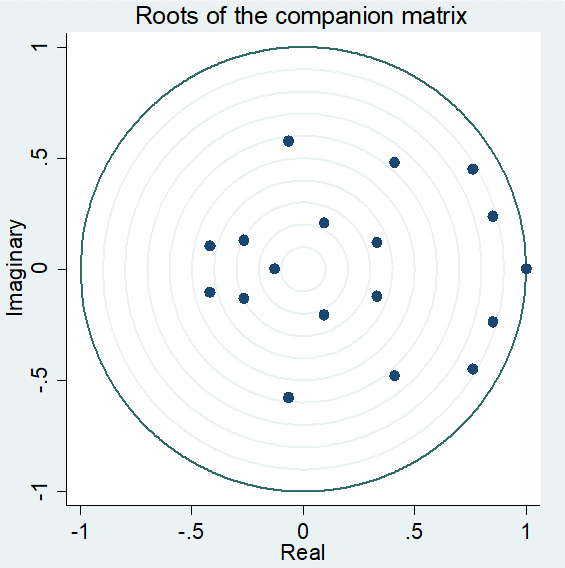
\includegraphics[width=.85\textwidth]{./img/P10_Obrazek_1}
\caption{\scriptsize Graphical representation of the stability condition (example): If the moduli of the eigenvalues of $\bm{A}_1$ are less than one, then the VAR($p$)-process is stable.}
\end{figure}
\end{minipage}
\end{frame}
%---------------------------------
\begin{frame}{VAR: Model setup and testing}
\underline{VAR model testing (residuals):}
\vspace*{4mm}
\begin{itemize}
\item Serial correlation tests: Portmanteau, Breusch \& Godfrey
\item Heteroskedasticity: ARCH
\item Normality tests: Jarque \& Bera, etc.
\item Structural stability: CUSUM \\
\vspace{0.5cm}
Functions \textbf{\textcolor{Gray}{serial()}}, \textbf{\textcolor{Gray}{arch()}}, \textbf{\textcolor{Gray}{normality()}} and \textbf{\textcolor{Gray}{stability()}} in package \textbf{\textcolor{Gray}{\{vars\}}}.
\end{itemize}
\end{frame}
%---------------------------------
\section{VAR: Forecasting}
\begin{frame}{VAR: Forecasting}
\textbf{VAR-based Forecasting: Introduction}\\
\vspace*{4mm}
\underline{Wold decomposition of stable VAR($p$) models:}\\
\vspace*{1mm}
\dots concept useful for forecasting and IRF construction. \\
\vspace*{3mm}
A simplified stable VAR($p$) model $\bm{y}_t = \bm{A}_1 \bm{y}_{t-1} + \bm{A}_2 \bm{y}_{t-2} + \dots + \bm{A}_p \bm{y}_{t-p} + \bm{u}_t$ ~can be written as: \\
\vspace{0.3cm}
$\bm{y}_t = \bm{\Phi}_0 \bm{u}_t + \bm{\Phi}_1 \bm{u}_{t-1} + \bm{\Phi}_2 \bm{u}_{t-2} \dots $ ~~,\\
\vspace*{3mm}
where $\bm{\Phi}_s = \sum_{j=1}^{s} \bm{\Phi}_{s-j} \bm{A}_j $ for $s = 1,2,\dots$; $\bm{A}_j = \bm{0}$ for $j > p$\\
\vspace*{2mm}
\qquad \quad $\bm{\Phi}_0 = \bm{I}_m$ $(m \times m)$ Identity matrix.\\
\vspace*{3mm}
See Lütkepohl: ``New introduction to multiple time series analysis'' for derivation and discussion.
\end{frame}
%---------------------------------
\begin{frame}{VAR: Forecasting}
\underline{Wold decomposition examples:}\\
\vspace*{3mm}
\begin{minipage}[t]{.43\textwidth}
\footnotesize
Stable VAR($2$) model:\\
\dots simplified: no intercept term

\vspace*{1mm}
$\bm{y}_t = \bm{A}_1 \bm{y}_{t-1} + \bm{A}_2 \bm{y}_{t-2} + \bm{u}_t$\\
may be written as:
\begin{flalign*}
\bm{y}_t & = \bm{\Phi}_0 \bm{u}_t + \bm{\Phi}_1 \bm{u}_{t-1} + && \\
& + \bm{\Phi}_2 \bm{u}_{t-2} \dots &&
\end{flalign*}

where:\\
$\bm{\Phi}_0 = \bm{I}_m$\\
$\bm{\Phi}_1 = \bm{\Phi}_0 \bm{A}_1$ \\
$\bm{\Phi}_2 = \bm{\Phi}_1 \bm{A}_1 + \bm{\Phi}_0 \bm{A}_2$ \\
$\bm{\Phi}_3 = \bm{\Phi}_2 \bm{A}_1 + \bm{\Phi}_1 \bm{A}_2$ \\
\dots \\
$\bm{\Phi}_s = \bm{\Sigma}_{j=1}^s \bm{\Phi}_{s-j} \bm{A}_j = $ \\
\hspace*{4mm} $ = \bm{\Phi}_{s-1} \bm{A}_1 + \bm{\Phi}_{s-2} \bm{A}_2$\\

\vspace*{-1.5mm}
($s=1,2, \dots$; $\bm{A}_j = \bm{0}$ for $j>p$)
\end{minipage}%
\qquad{\color{Blue}\vrule}\qquad
\begin{minipage}[t]{.42\textwidth}
\footnotesize
Stable VAR($1$) model:\\
\dots any VAR($p$) may be written as VAR($1$)

\vspace*{1mm}
$\bm{y}_t = \bm{A}_1 \bm{y}_{t-1} + \bm{u}_t$\\
may be written as: 
\begin{flalign*}
\bm{y}_t & = \bm{\Phi}_0 \bm{u}_t + \bm{\Phi}_1 \bm{u}_{t-1} + && \\
& + \bm{\Phi}_2 \bm{u}_{t-2} \dots &&
\end{flalign*}

where:\\
$\bm{\Phi}_0 = \bm{I}_m$\\
$\bm{\Phi}_1 = \bm{\Phi}_0 \bm{A}_1 = \bm{A}_1$ \\
$\bm{\Phi}_2 = \bm{\Phi}_1 \bm{A}_1 = \bm{A}_1 \bm{A}_1 = \bm{A}_1^2$ \\
$\bm{\Phi}_3 = \bm{\Phi}_2 \bm{A}_1 = \bm{A}_1^3$ \\
\dots \\
$\bm{\Phi}_s = \bm{A}_1^s$\\

\vspace*{-1.5mm}
(note that $\bm{\Phi}_0 =  \bm{A}_1^0 = \bm{I}_m$)
\end{minipage}
\end{frame}
%---------------------------------
\begin{frame}{VAR: Forecasting}
\small
\textbf{Iterative forecasting}\\
\vspace*{1mm}
VAR($p$) model is estimated using observations $t = 1, 2, \dots, T$:\\
\vspace*{1mm}
\qquad $\bm{y}_t = \hat{\bm{A}}_1 \bm{y}_{t-1} + \hat{\bm{A}}_2 \bm{y}_{t-2} + \dots + \hat{\bm{A}}_p \bm{y}_{t-p} + \hat{\bm{u}}_t$ \\
\vspace*{2mm}
and for $t = T$: \\
\vspace*{2mm}
\qquad $\bm{y}_T = \hat{\bm{A}}_1 \bm{y}_{T-1} + \hat{\bm{A}}_2 \bm{y}_{T-2} + \dots + \hat{\bm{A}}_p \bm{y}_{T-p} + \hat{\bm{u}}_T$.\\
\vspace*{2mm}
Arbitrarily long forecasts ($t = T + 1, T+2, \dots, T+h$) can be iteratively produced using the estimated $\bm{A}$-matrices and the observed ($t=1,2,\dots,T$) and predicted ($t = T \! + \! 1, T\! + \! 2, \dots, T\!+\!h$) values of $\bm{y}_t$: \\
\vspace*{5mm}
$\hat{\bm{y}}_{T+1} = \hat{\bm{A}}_1 \bm{y}_{T} + \hat{\bm{A}}_2 \bm{y}_{T-1} + \dots + \hat{\bm{A}}_p \bm{y}_{T-p+1}$\\
$\hat{\bm{y}}_{T+2} = \mytikzmark{a}{\circledd{$\hat{\bm{A}}_1 \hat{\bm{y}}_{T+1}$}} + \hat{\bm{A}}_2 \bm{y}_{T} + \dots + \hat{\bm{A}}_p \bm{y}_{T-p+2}$\\
$\hat{\bm{y}}_{T+3} = \mytikzmark{b}{\circledd{$\hat{\bm{A}}_1 \hat{\bm{y}}_{T+2}$}} + \mytikzmark{c}{\circledd{$\hat{\bm{A}}_2 \hat{\bm{y}}_{T+1}$}} + \dots + \hat{\bm{A}}_p \bm{y}_{T-p+3}$\\
\dots\dots
\begin{tikzpicture}[<-,overlay,remember picture,inner sep=1.5pt,shorten <=0.2em,font=\scriptsize]
\tikzset{
    mynode/.style={rectangle,draw=ProcessBlue, fill=White, semithick, inner sep=.2em, minimum size=2em, text centered, text width=11em},
    myarrow/.style={->, >=stealth, thin, ProcessBlue}
}
\node[mynode] at (8.5,2.2) (Box){As we move through the prediction time period, predicted values are used as regressors for subsequent periods \& predictions \dots};
  \draw[myarrow] (Box) -- ++   (a);
  \draw[myarrow] (Box) -- ++   (b);
  \draw[myarrow] (Box) -- ++   (c);
\end{tikzpicture}
\end{frame}
%---------------------------------
\begin{frame}{VAR: Forecasting}
\textbf{Forecast error covariance matrix:}\\
\tiny
\begin{flalign*}
\textit{cov} \bigg(
\begin{bmatrix}
    \bm{y}_{T+1} - \hat{\bm{y}}_{T+1} \\
    \dots \\
    \bm{y}_{T+h} - \hat{\bm{y}}_{T+h} \\
\end{bmatrix}
\bigg) =
\begin{bmatrix}
   \bm{I} & \bm{0} & \dots & \bm{0} \\
   \bm{\Phi} & \bm{I} & & \bm{0} \\
   \vdots & & \ddots & \bm{0}\\
   \bm{\Phi}_{h-1} & \bm{\Phi}_{h-2} & \dots & \bm{I} \\
\end{bmatrix}
(\bm{\Sigma}_u \otimes \bm{I}_h)
\begin{bmatrix}
   \bm{I} & \bm{0} & \dots & \bm{0} \\
   \bm{\Phi}_1 & \bm{I} & & \bm{0} \\
   \vdots & & \ddots & \bm{0}\\
   \bm{\Phi}_{h-1} & \bm{\Phi}_{h-2} & \dots & \bm{I} \\
\end{bmatrix}^\prime
\end{flalign*}
\begin{minipage}[c][.1\textheight][s]{.3\textwidth}
\vspace*{-2cm}
{\footnotesize
where \\
$\bm{\Sigma}_u = \textit{cov }(\bm{u}_t) $ is the white noise covariance matrix,\\
\smallskip
($\bm{\Sigma}_u \otimes \bm{I}_h$) is a Kroneker product; \\
\smallskip
$\bm{I}_h$ is $h \times h$, \\ 
\smallskip
$\bm{\Phi}_i$ are the coefficient matrices of the Wold moving average representation of a stable VAR($p$)-process.}
\end{minipage}
\hspace*{4mm}
\begin{minipage}[s]{.49\textwidth}
\begin{figure}
\centering
\caption{\scriptsize \textbf{Forecast from a VAR($5$): example} (confidence levels included)}
\vspace*{-2mm}
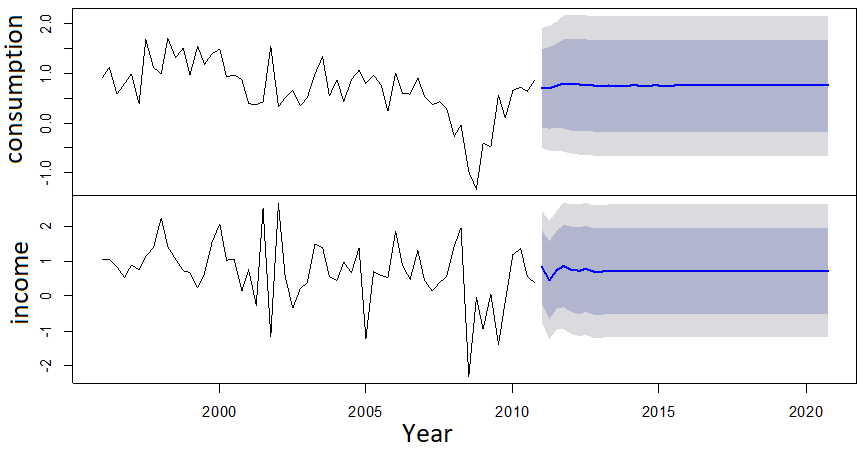
\includegraphics[width=1.4\textwidth]{./img/P10_Obrazek_2}\\
\end{figure}
\end{minipage}
\end{frame}
%---------------------------------
\section{VAR: Impulse-response functions (IRFs)}
\begin{frame}{VAR: Impulse-response functions (IRFs)}
\small
Based on Wold decomposition of a stable VAR($p$).\\
\vspace*{3mm}
IRFs describe the dynamic interactions between endogenous variables. (provided $\bm{y}_t$ is stationary!)\\
\vspace*{3mm}
The $[i, j]$-th elements of the matrices $\bm{\Phi}_s$ are (interpreted as) the expected response of variable $y_{(i,t+s)}$ to a unit change in variable $y_{j,t}$.\\
\vspace*{3mm}
IRF can be cumulated through time: $[i, j]$-th elements of  $\bm{C}_s = \sum_{l=1}^s \bm{\Phi}_l$ measure the accumulated response of variable $y_{i, t+s}$ to a unit change in variable $y_{j,t}$.\\
\vspace*{3mm}
IRFs are used for policy analysis: for individual shocks (shocks in different model equations), we can study the dynamic effects on all variables in the model.\\
\vspace*{3mm}
Disturbances in different model equations tend to be  contemporaneously correlated: we cannot realistically simulate isolated shocks. Solution: model transformation/orthogonalization\dots
\end{frame}
%---------------------------------
\begin{frame}{VAR: Impulse-response functions (IRFs)}
\small 
\textbf{IRF example:}\\
(from Lütkepohl: ``New introduction to multiple time series analysis'')\\
\vspace*{5mm}
We start with an estimated $3$-dimensional VAR($1$) system:\\
\vspace*{3mm}
\begin{minipage}[t]{.3\textwidth}
\begin{flalign*}
y_{1,t} & = 0.5 y_{1,t-1}  && \\
y_{2,t} & = 0.1 y_{1,t-1}  && \\
y_{3,t} & =  && 
\end{flalign*}
\end{minipage}
\hspace*{-1.1cm}
\begin{minipage}[t]{.3\textwidth}
\begin{flalign*}
& + u_{1,t} && \\
+ \ 0.1 y_{2,t-1} + 0.3 y_{3,t-1} & + u_{2,t} && \\
+ \ 0.2 y_{2,t-1} + 0.3 y_{3,t-1} & + u_{3,t} &&
\end{flalign*}
\end{minipage}

\small 
This may be re-written as \\
{\scriptsize
\begin{flalign*}
\begin{bmatrix}
    y_{1,t} \\
    y_{2,t} \\
    y_{3,t} \\
\end{bmatrix}
=
\begin{bmatrix}
   0.5 & 0 & 0 \\
   0.1 & 0.1 & 0.3 \\
   0 & 0.2 & 0.3 \\
\end{bmatrix}
\begin{bmatrix}
   y_{1,t-1} \\
   y_{2,t-1} \\
   y_{3,t-1} \\
\end{bmatrix}
+
\begin{bmatrix}
   u_{1,t} \\
   u_{2,t} \\
   u_{3,t} \\
\end{bmatrix} &&
\end{flalign*}}
\vspace*{-2mm}
\begin{flalign*}
{\small  \textnormal{Hence, }} {\scriptsize \bm{A}_1 =
\begin{bmatrix}
   0.5 & 0 & 0 \\
   0.1 & 0.1 & 0.3 \\
   0 & 0.2 & 0.3 \\
\end{bmatrix}}
{\small \textnormal{ Also, for a VAR(1) model: } \bm{\Phi}_s = \bm{A}_1^s} &&
\end{flalign*}
\begin{tikzpicture}[<-,overlay,remember picture,inner sep=1.5pt,shorten <=0.2em,font=\footnotesize]
\tikzset{
    mynode/.style={rectangle,draw=Red, very thick, inner sep=.5em, minimum size=2em, text width=10em}
}
\node[mynode] at (9.3,3.5) (How){\underline{How IRFs work:} \\
Say, at time $t$, we have a unit disturbance in $y_{2,t}$ (\underline{\textbf{isolated}} contemporaneous disturbance through $u_{2,t}$). At time $t+1$, it causes: $y_{2,t+1}$ changes by 0.1 and $y_{3,t+1}$ changes by 0.2 and $y_{1,t+1}$ is unaffected
};
\tikzset{
    mynode/.style={rectangle,draw=Red, dashed, thick, inner sep=0em, minimum size=4em, text centered, text width=2.3em},
    myarrow/.style={->, >=stealth, thin, Red}
}
\node[mynode] at (3.4,4.8) (1){};
\draw[myarrow] (1) -- ++ (How);
	\tikzset{
   	 mynode/.style={rectangle,draw=Red, dashed, thick, inner sep=0em,  minimum width=0.5cm, 		 minimum height = 1.1cm},
    	 myarrow/.style={->, >=stealth, thin, Red}
}
	\node[mynode] at (2.4,2.6) (2){};
	\draw[myarrow] (2) -- ++ (How);
\end{tikzpicture}
\end{frame}
%---------------------------------
\begin{frame}{VAR: Impulse-response functions (IRFs)}
\small 
\textbf{IRF example contd.}\\
Using $\bm{\Phi}_s = \bm{A}_1^s$, the IRFs may be generated as follows:
\begin{minipage}[t]{.4\textwidth}
{\scriptsize
\begin{align*}
\bm{\Phi}_0 & = \bm{A}_1^0 =
\begin{bmatrix}
1 & 0 & 0 \\
0 & 1 & 0 \\
\mytikzmark{a}{\circled{$0$}} & 0 & 1 \\
\end{bmatrix}, \\
\bm{\Phi}_1 & = \bm{A}_1 =
\begin{bmatrix}
0.500 & 0 & 0 \\
0.100 & 0.100 & 0.300 \\
\mytikzmark{b}{\circled{$0$}} & 0.200 & 0.300 \\
\end{bmatrix}, \\
\bm{\Phi}_2 & = \bm{A}_1^2 =
\begin{bmatrix}
0.250 & 0 & 0 \\
0.060 & 0.070 & 0.120 \\
\mytikzmark{c}{\circled{$0.020$}} & 0.080 & 0.150 \\
\end{bmatrix}, \\
\bm{\Phi}_3 & = \bm{A}_1^3 =
\begin{bmatrix}
0.125 & 0 & 0 \\
0.037 & 0.031 & 0.057 \\
\mytikzmark{d}{\circled{$0.018$}} & 0.038 & 0.069 \\
\end{bmatrix}, \\
\dots
\end{align*}}
\end{minipage}
\hspace*{1mm}
\begin{minipage}[t]{.49\textwidth}
\begin{figure}
\centering
\mytikzmark{F}{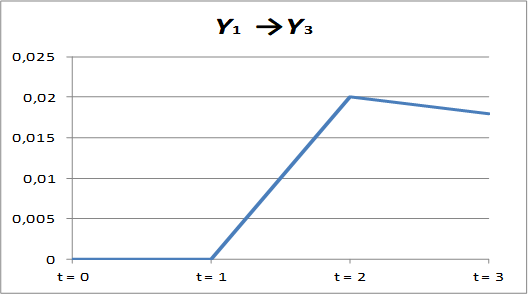
\includegraphics[width=5.1cm, height=3.5cm]{./img/P10_Obrazek_3}}
\end{figure}
\end{minipage}
\begin{tikzpicture}[<-,overlay,remember picture,inner sep=1.5pt,shorten <=0.2em,font=\scriptsize]
\tikzset{
    mynode/.style={rectangle,draw=Red, thick, inner sep=0.22em, minimum size=4em, text width=14em},
    myarrow/.style={->, >=stealth, thin, Red}
}
\node[mynode] at (8.1,2.3) (E){[3,1]-th elements of $\bm{\Phi}_s = \bm{A}_1^s$ 
[VAR(1) model \dots] matrices measure the response of variable $y_{3, t+s}$ to a unit change in variable $y_{1,t}$ (a unit $u_{1,t}$ disturbance occurs at $t=0$). \\
\textbf{$\bm{\Phi_s}$: ``Impulses/shocks in columns and responses in rows''}
};
\draw[myarrow] (a) -- ++ (F);
\draw[myarrow] (b) -- ++ (F);
\draw[myarrow] (c) -- ++ (F);
\draw[myarrow] (d) -- ++ (F);
\end{tikzpicture}
\end{frame}
%---------------------------------
\begin{frame}{VAR: Impulse-response functions (IRFs)}
\small 
\textbf{IRF example contd.}\\
Cumulative IRFs may be easily produced and plotted using $\bm{C}_s = \sum_{l=1}^s \bm{\Phi}_l$: \\
\medskip
\begin{minipage}[t]{.45\textwidth}
\qquad {\scriptsize IRF (CPI $\to$ GDP)} \\
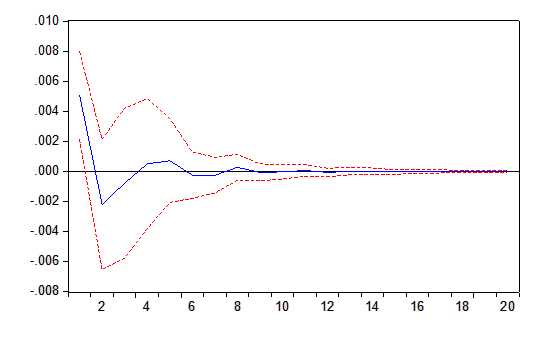
\includegraphics[width=\textwidth]{./img/P10_Obrazek_4}
\end{minipage}
\begin{minipage}[t]{.45\textwidth}
\qquad {\scriptsize Cumulative IRF (CPI $\to$ GDP)} \\
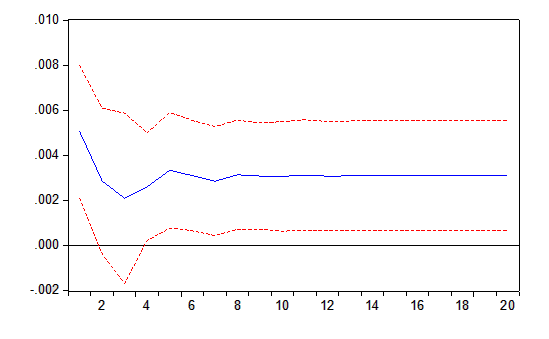
\includegraphics[width=1.04\textwidth]{./img/P10_Obrazek_5}
\end{minipage}\\
\medskip
In a stable VAR($p$) model, responses to a one-off shock die out over time (shown left). Hence, the accumulated IRF converges to some constant value (shown right). \\
\medskip
{\footnotesize
Important extensions to VARs are based on assumptions (zero restrictions) on the (asymptotic) behavior of $\bm{C}_s$ (Blanchard-Quah decomposition, see: Lütkepohl: ``New introduction to multiple time series analysis'')}
\end{frame}
%---------------------------------
\begin{frame}{VAR: Impulse-response functions (IRFs)}
\small 
\textbf{IRF – orthogonalization example}\\
\medskip
Previous example is based on – a very strong – assumption of uncorrelated random effects. Usually, we cannot realistically simulate isolated shocks on observed variables. \\
\medskip
2-dimensional VAR(1) model with correlated errors example:
\begin{flalign*}
\begin{bmatrix}
y_{1t} \\
y_{2t} \\
\end{bmatrix}
=
\begin{bmatrix}
a_{11} & a_{12} \\
a_{21} & a_{22} \\
\end{bmatrix}
\begin{bmatrix}
y_{1t-1} \\
y_{2t-1} \\
\end{bmatrix}
+
\begin{bmatrix}
u_{1t} \\
u_{2t} \\
\end{bmatrix} &&
\end{flalign*}
where $\textit{var}(u_{1t}) = \sigma_1^2$ and $\textit{var}(u_{2t}) = \sigma_2^2$,\\
and, most importantly, $\mytikzmark{A}{\begingroup \color{Red}
      \underbrace{\color{Black} \textit{cov}(u_{1t}, u_{2t}) = E(u_{1t} \cdot u_{2t}) = \textit{cov}_{12} \neq 0} \endgroup }$. \\
\medskip
$\Rightarrow$ It is unrealistic to simulate isolated unit disturbances to $\bm{u}_t$ as {\scriptsize $\begin{bmatrix}
1 \\ 0 
\end{bmatrix}$}. \\
\medskip
If $\textit{cov}_{12} \neq 0$, then – for a unit disturbance ~in $u_{1t}$ – we have: ${\scriptsize\textit{dist}(\bm{u}_t) = 
\begin{bmatrix}
1\\ E(1 \cdot u_{2t})
\end{bmatrix}
= \mytikzmark{B}{
\begin{bmatrix}
1\\ \textit{cov}_{12}
\end{bmatrix}}}$
\begin{tikzpicture}[<-,overlay,remember picture,inner sep=1.5pt,shorten <=0.2em,font=\scriptsize]
\tikzset{
    myarrow/.style={->, >=stealth, semithick, Red}
}
\draw[myarrow, to path={|- (\tikztotarget)}]
  (A) edge (B);
\end{tikzpicture}
\end{frame}
%---------------------------------
\begin{frame}{VAR: Impulse-response functions (IRFs)}
\small 
\textbf{IRF – orthogonalization example contd.}\\
\vspace{0.3cm}
Base VAR model: $ {\scriptsize \begin{bmatrix}
y_{1t} \\
y_{2t} \\
\end{bmatrix}
=
\begin{bmatrix}
a_{11} & a_{12} \\
a_{21} & a_{22} \\
\end{bmatrix}
\begin{bmatrix}
y_{1t-1} \\
y_{2t-1} \\
\end{bmatrix}
+
\begin{bmatrix}
u_{1t} \\
u_{2t} \\
\end{bmatrix}}$ \\
\vspace{0.4cm}
In our VAR(1) model, responses to a unit disturbance in $u_{1t}$ are: \\
\vspace{0.4cm}
For a $\bm{u}_t$ disturbance $ {\scriptsize \begin{bmatrix}
1 \\ 0
\end{bmatrix}}$: \quad $ {\scriptsize E \Delta \begin{bmatrix}
y_{1t+1} \\ y_{2t+1}
\end{bmatrix}
=
\begin{bmatrix}
a_{11} & a_{12} \\
a_{21} & a_{22} \\
\end{bmatrix}
\begin{bmatrix}
1 \\ 0
\end{bmatrix}
=
\begin{bmatrix}
a_{11} \\ a_{21}
\end{bmatrix}}$ \\
\medskip
For a $\bm{u}_t$ disturbance $ {\scriptsize \begin{bmatrix}
1 \\ \textit{cov}_{12}
\end{bmatrix}}$: \\
$$ {\scriptsize E \Delta \begin{bmatrix}
y_{1t+1} \\ y_{2t+1}
\end{bmatrix} 
=
\begin{bmatrix}
a_{11} & a_{12} \\
a_{21} & a_{22} \\
\end{bmatrix}
\begin{bmatrix}
1 \\ \textit{cov}_{12}
\end{bmatrix}
=
\begin{bmatrix}
a_{11} + a_{12} \textit{cov}_{12} \\
a_{21} + a_{22} \textit{cov}_{12} \\
\end{bmatrix}}$$ \\
\vspace*{1cm}
\begin{tikzpicture}[<-,overlay,remember picture,inner sep=1.5pt,shorten <=0.2em,font=\small]
\tikzset{
    mynode/.style={rectangle,draw=Red, dashed, thick, inner sep=0.22em, minimum size=2.2em, text width=6.05em}
}
\node[mynode] at (8,1.72) (O){};
\tikzset{
    mynode/.style={rectangle, minimum size=5em, inner sep=-1em, text width=30.8em},
    myarrow/.style={->, >=stealth, thick, Red}
}
\node[mynode] at (5.45,0.2) (H){It is virtually impossible to study the isolated effects of individual disturbances (analysis is even more complicated for $p > 1$ \& $m > 2$)};
\draw[myarrow] (H) -- ++ (O);
\end{tikzpicture}
\end{frame}
%---------------------------------
\begin{frame}{VAR: Impulse-response functions (IRFs)}
\textbf{IRF – orthogonalization example contd.}\\
\bigskip
Our sample VAR(1) model: $ {\small \begin{bmatrix}
y_{1t} \\
y_{2t} \\
\end{bmatrix}
=
\begin{bmatrix}
a_{11} & a_{12} \\
a_{21} & a_{22} \\
\end{bmatrix}
\begin{bmatrix}
y_{1t-1} \\
y_{2t-1} \\
\end{bmatrix}
+
\begin{bmatrix}
u_{1t} \\
u_{2t} \\
\end{bmatrix}}$ \\
\medskip
with $\textit{var}(u_{1t}) = \sigma_1^2$, $\textit{var}(u_{2t}) = \sigma_2^2$ and $\textit{cov}_{12} \neq 0$, \\ errors may be transformed (orthogonalized) as follows: 
\begin{align*}
{\small 
\begin{bmatrix}
y_{1t} \\
(y_{2t} - \delta y_{1t}) \\
\end{bmatrix}
=
\begin{bmatrix}
a_{11} & a_{12} \\
(a_{21} - \delta a_{11}) & (a_{22} - \delta a_{12})\\
\end{bmatrix}
\begin{bmatrix}
y_{1t-1} \\
y_{2t-1} \\
\end{bmatrix}
+
\begin{bmatrix}
u_{1t} \\
(u_{2t} - \delta u_{1t}) \\
\end{bmatrix}}
\end{align*}
where $\delta = \textit{cov}_{12}/\sigma_1^2$ \quad and \quad $\textit{cov}(u_{1t}, (u_{2t} - \delta u_{1t})) = 0$ \\
\bigskip
Hence, IRFs based on the \underline{\textbf{transformed model}} depict the isolated effects of a given unit disturbance.
\end{frame}
%---------------------------------
\begin{frame}{VAR: Impulse-response functions (IRFs)}
\small
\textbf{IRF orthogonalization – a generalized approach \& notation:}\\
\bigskip
In a VAR($p)$ model, $\bm{\Sigma}_u = \textit{cov}(\bm{u}_t)$ is the error-term covariance matrix and it may be expressed as $\bm{\Sigma}_u =\bm{PP'}$ where $\bm{P}$ is a lower triangular matrix (assumptions on $\bm{\Sigma}_u$ apply).\\
\medskip
Orthogonalized IRFs from a VAR($p$) model $\bm{y}_t = \bm{A}_1 \bm{y}_{t-1} + \bm{A}_2 \bm{y}_{t-2} + \dots + \bm{A}_p \bm{y}_{t-p} + \bm{u}_t$ \\may be calculated using the transformed MA representation:\\
\medskip
$\bm{y}_t = \bm{\Psi}_0 \bm{\varepsilon}_t + \bm{\Psi}_1 \bm{\varepsilon}_{t-1} + \bm{\Psi}_2 \bm{\varepsilon}_{t-2} \dots$, \\
\medskip
where: $\bm{\varepsilon}_t = \bm{P}^{-1} \bm{u}_t$\\
\hspace*{9mm} $\bm{\Psi}_i = \bm{\Phi}_i \bm{P}$ for $i=1,2,\dots$\\
\hspace*{8.7mm} $\bm{\Psi}_0 = \bm{P}$. \\
\medskip
(Use bootstrapped confidence intervals for the orthogonalized IRFs)\\
\dots see: Lütkepohl: ``New introduction to multiple time series analysis'' for detailed description. 
\end{frame}
%---------------------------------
\begin{frame}{VAR: Impulse-response functions (IRFs)}
\textbf{IRF orthogonalization – final remarks:}\\
\medskip
\begin{itemize}
\item $\bm{\Sigma}_u = \bm{PP'}$ and $\bm{P}$–based transformation is sensitive to the ordering of equations.\\
i.e. different ordering of variables in $\bm{y}$ often yields different orthogonalized IRFs! \\
\medskip
\item Orthogonalized innovations are difficult to interpret... Even if $y_{1t}$ and $y_{2t}$ are well defined, the dimension of ($y_{2t}-\delta y_{1t}$) / see previous example / often has no economic interpretation.\\
\medskip
We treat orthogonalized IRFs as dimensionless series \dots \\
\medskip
\item Generalized orthogonalization approaches exist (IRFs independent of $\bm{y}$ ordering). \\
\dots see: Lütkepohl: ``New introduction to multiple time series analysis''
\end{itemize}
\end{frame}
%---------------------------------
\section{VAR: Variance decomposition}
\begin{frame}{VAR: Variance decomposition}
\textbf{Forecast Error Variance Decomposition (FEVD)}\\
\medskip
\begin{itemize}
\item FEVD: based on orthogonalised impulse response coefficient matrices $\bm{\Psi}$
\item Used to analyse the contribution of variable $j$ to the $h$-step FEV of variable $k$.
\item \textcolor{Blue}{\textbf{R}}: use \textbf{\textcolor{Gray}{fevd()}} in \textbf{\textcolor{Gray}{\{vars\}}}
\end{itemize}
\vspace*{-6mm}
\begin{figure}
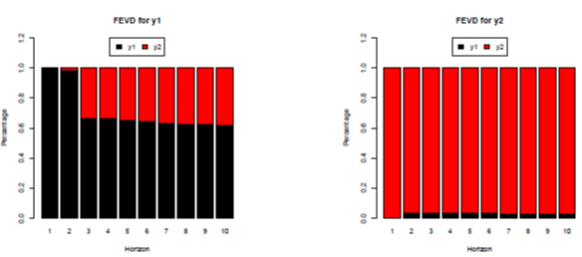
\includegraphics[width=\textwidth, height=4.1cm]{./img/P10_Obrazek_6}
\end{figure}
\end{frame}
%---------------------------------
\begin{frame}{VAR: Final remarks}
\textbf{Are VAR models atheoretical?}\\
\begin{itemize}
\item Essentially yes, there are no prior restrictions on parameters in VARs.
\item Often, estimated VARs may lead to models consistent with economic theory. For example, for $\bm{y}_t^{\prime} = (\textit{Unempl}_t, \textit{CPI}_t)$, VAR($p$) models often generate IRFs consistent with Phillip’s theory. For verification, we use causality tests.\\
\end{itemize}
\medskip
\textbf{IRF critique}\\
\begin{itemize}
\item If ``important'' variables are dropped from a VAR model,\\IRFs may be significantly distorted.
\item In most practical cases (yet, not generally) predictions from such ``reduced'' VARs might remain largely unaffected.
\end{itemize}
\end{frame}
%---------------------------------
\begin{frame}{VAR: Final remarks}
\textbf{Selected VAR-related topics \& extensions \\not covered in this course:}\\
\begin{itemize}
\item Structural VAR models: SVARs
\item Time-varying (and/or) factor-augmented VARs
\item Blanchard-Quah decomposition
\item \dots many extensions to VARs exist
\end{itemize}
\end{frame}
%---------------------------------
\section{VECM}
\begin{frame}{VECM: Introduction}
\begin{itemize}
\item VAR models are well suited to model systems of nonstationary cointegrated variables.
	\begin{itemize}
	\item Forecasting is possible, 
    \item IRFs do not converge to zero over time if the underlying series are non-stationary \dots
	\end{itemize}
\item For cointegrated series, we can use the error correction mechanism (ECM) to model short-time dynamics. 
\item Such models are named Vector Error Correction Models (VECMs). \\
\vspace{0.1cm}	
Long term dynamics in the $m$-dimensional system of variables [given cointegrating relationship(s) exist(s)] is used in a VECM: an ECM-like model in first differences.
	
\item Most of the previous discussion of VAR models can be adequately applied to VECMs.
\item VECM-specific topics follow
\end{itemize}
\end{frame}
%---------------------------------
\begin{frame}{VECM: Number of cointegrating vectors}
\footnotesize
For an $m$-dimensional $I$(1) / non-stationary / vector $\bm{y}=(y_1, y_2, \dots, y_m)'$, there are
\begin{itemize}
\item $0 < r < m$ possible cointegrating vectors [$r=0$ $\Rightarrow$ non-CI series]
\item and ($m-r$) common stochastic trends.\\
(Proof comes from a Beveridge-Nelson decomposition of $\Delta y$)
\end{itemize}
$\bm{y} = (y_1, y_2)'$: max. 1 linearly independent cointegrating vector: $r \in \{0;1\}$
\begin{itemize}
\item If any $(\alpha y_1 + \beta y_2) \sim I(0)$, we can find $\infty$ linear combinations of $(\alpha, \beta)$ that lead to a $I(0)$ processes.
\item Hence, it is easy and common to normalize the CI relationship by setting $\alpha=1$
\item If $y_1, y_2 \sim CI(1,1)$, a cointegrating vector $\bm{\beta} = (1, -\beta_2)'$ exists, such that $(y_1 - \beta_2 y_2) \sim I(0)$
\end{itemize}
Example of a CI system for $\bm{y} = (y_1, y_2)'$ with $\bm{\beta} = (1, -\beta_2)'$:
\begin{enumerate}[ {[}1{]} ]
\item $y_{1t} = \beta_2 y_{2t} + u_t$, \qquad $\Leftarrow$ one CI relationship
\item $y_{2t} = y_{2t-1} + v_t$, \qquad $\Leftarrow$ one common ``stochastic trend''\\
where $u_t, v_t \sim I(0)$
\end{enumerate}
\end{frame}
%---------------------------------
\begin{frame}{VECM: Number of cointegrating vectors}
\footnotesize
Ex.: CI system for $\bm{y} = (y_1, y_2, y_3)'$ with $r=1$ an $\bm{\beta} = (1, -\beta_2, -\beta_3)'$:
\begin{enumerate}[ {[}1{]} ]
\item $y_{1t} = \beta_2 y_{2t} + \beta_3 y_{3t} + u_t$, \  $\Leftarrow$ one CI relationship
\item $y_{2t} = y_{2t-1} + v_t$, \hspace*{1.20cm} $\Leftarrow$ first common ``stochastic trend''
\item $y_{3t} = y_{3t-1} + w_t$, \hspace*{1.12cm} $\Leftarrow$ second common ``stochastic trend''\\
where $u_t, v_t, w_t \sim I(0)$
\end{enumerate}
The $1^{st}$ equation describes the long-run equilibrium, $2^{nd}$ and $3^{rd}$ equations describe the ($m-r$) common stochastic trends.\\
\medskip
Possible economic setup for the example:\\
\medskip
$y_{1t} \sim I(1)$ nominal F/X rate index for 2 currencies (domestic/foreign), \\ 
$y_{2t} \sim I(1)$ domestic inflation index (e.g. CPI), \\
$y_{3t} \sim I(1)$ foreign inflation. \\
\medskip
We can test a hypothesis of stationary combination of the three series:\\  real exchange rate $\sim I(0)$: under $H_0$: $\bm{\beta} = (1, -1, -1)'$ \\ \dots i.e. the 2 identifying CI restrictions imposed are: $\beta_2 = \beta_3 = 1$ 
\end{frame}
%---------------------------------
\begin{frame}{VECM: Number of cointegrating vectors}
\footnotesize
Example of a CI system for $\bm{y} = (y_1, y_2, y_3)'$ with $r=2$
\begin{enumerate}[ {[}1{]} ]
\item $y_{1t} = \beta_{13} y_{3t} + u_t$, \quad  $\Leftarrow$ first CI relationship
\item $y_{2t} = \beta_{23} y_{3t} + v_t$, \quad  $\Leftarrow$ second CI relationship
\item $y_{3t} = y_{3t-1} + w_t$, \hspace*{2.87mm} $\Leftarrow$ a common ``stochastic trend''\\
where $u_t, v_t, w_t \sim I(0)$
\end{enumerate}
Here, we have two CI vectors: $\bm{\beta}_1 = (1,0,-\beta_{13})'$ and $\bm{\beta}_2 = (0,1, -\beta_{23})'$. \\
\medskip
\textcolor{Blue}{Remember:} \quad $\bm{\beta}_1$ and $\bm{\beta}_2$ are normalized - yet not unique - stationary \\ \hspace*{2cm} combinations of the variables. \\
\smallskip
\hspace*{2cm} Any linear combination: $\bm{\beta}_3 = c_1 \bm{\beta}_1 + c_2 \bm{\beta}_2$ is also a CI vector \\
\smallskip
\hspace*{2cm} \textcolor{Blue}{ $\bm{\beta}_1$ and $\bm{\beta}_2$ form the basis (span the space) of \\ \hspace*{2cm} cointegrating vectors\dots}\\
\medskip
Financial market-based setup for the example:\\
$y_{1t} \sim I(1)$ Long-term interest rate ``1''   (say, 3M), \\ 
$y_{2t} \sim I(1)$ Long-term interest rate ``2''   (say, 6M), \\
$y_{3t} \sim I(1)$ Short-term interest rate (say, overnight).\\
\medskip
CI relationships indicate that the spreads between the short-run and long-run rates are stationary, i.e. $I(0)$.
\end{frame}
%---------------------------------
\begin{frame}{VECM: Construction}
\footnotesize
Start with a VAR($p$) model for an $m$-dimensional $I(1)$ / non-stationary / vector $\bm{y} = (y_1, y_2, \dots, y_m)'$: \\
$\bm{y}_t = \bm{\Theta} \bm{D}_t + \bm{A}_1 \bm{y}_{t-1} + \bm{A}_2 \bm{y}_{t-2} + \dots + \bm{A}_p \bm{y}_{t-p} + \bm{u}_t$, \qquad $t = 1,2,\dots,T$, \\
where $\bm{D}_t$ contains deterministic terms (constant, trend, seasonality, etc.)\\
\medskip
Even if $\bm{y}$ series are cointegrated through some CI vector $\bm{\beta}$, the cointegrating relationship is ``hidden'' in the VAR($p$) representation – it only becomes apparent in first differences-based VECM:\\
\medskip
The VECM model is defined as follows:\\
$\bm{\Delta}\bm{y}_t = \bm{\Theta} \bm{D}_t + \mytikzmark{K}{\circled{$\bm{\Pi} \bm{y}_{t-1}$}} + \bm{\Gamma}_1 \bm{\Delta} \bm{y}_{t-1} + \dots + \bm{\Gamma}_{p-1} \bm{\Delta} \bm{y}_{t-p+1} + \bm{\varepsilon}_t$, \\
\medskip
where \ $\bm{\Pi} = \bm{A}_1 + \bm{A}_2 + \dots + \bm{A}_p - \bm{I}_{m \times m}$ is the long-run impact matrix \\
\smallskip
\hspace*{1cm} $0 \leq$ rank$(\bm{\Pi}) < m$ defines $r$, the number of CI vectors\\
\smallskip
\hspace*{1cm} $\bm{\Gamma}_k = - \sum_{j=k+1}^p \bm{A}_j \quad k=1,\dots,p-1$ : short-run impact matrices\\
\medskip
Note that VAR($p$) is transformed into a ``VECM($p-1$)''

\begin{tikzpicture}[<-,overlay,remember picture,inner sep=1.5pt,shorten <=0.2em,font=\tiny]
\tikzset{
    mynode/.style={rectangle,draw=Red, thick, inner sep=0.2em, minimum size=2.2em, text width=9.65em},
    myarrow/.style={->, >=stealth, dotted, thick, Red}
}
\node[mynode] at (9.8,3.9) (H){This is the error correction element of the VECM specification};
\draw[myarrow] (H) -- ++ (K);
\end{tikzpicture}
\end{frame}
%---------------------------------
\begin{frame}{VECM: Construction}
\footnotesize
VAR(1) model for a 2-dimensional vector $\bm{y} = (y_1, y_2)'$; ~~~$y_1, y_2 \sim CI(1,1)$:\\
\vspace{0.2cm}
$\bm{y}_t = \bm{A}_1 \bm{y}_{t-1} + \bm{u}_t$, \qquad $t=1,2, \dots, T$, \\
\bigskip
For a bivariate VAR, only one cointegrating vector  $\bm{\beta}=(1, -\beta_2)'$  can exist /normalized/. The VECM model is defined as follows:\\
\medskip
$\Delta\bm{y}_t = \bm{\Pi} \bm{y}_{t-1} + \bm{\varepsilon}_t$, \\
\medskip
where $\bm{\Pi}$ is a $2 \times 2$ matrix with rank: $r=1$.\\
\hspace*{8mm} $\bm{\Pi}$ may be decomposed as follows: $\bm{\Pi} \!=\! \begin{pmatrix}
\alpha_1 \\ \alpha_2 
\end{pmatrix} \!
\left( 1, -\beta_2 \right) \! = \!\!
\begin{bmatrix}
\alpha_1 & \!\!  -\alpha_1 \beta_2 \\ 
\alpha_2 & \!\! -\alpha_2 \beta_2 \\
\end{bmatrix}$ \\
\medskip
To understand the decomposition, we may re-write the VECM: \\
\medskip
$\Delta y_{1t} = \alpha_1 (y_{1,t-1} - \beta_2 y_{2,t-1}) + \varepsilon_{1t}$ \\ 
\vspace{0.1cm}
$1^{st}$ equation relates changes in $y_{1t}$ to  disequilibrium error $(y_{1,t-1} \! - \! \beta_2 y_{2,t-1})$\\
\vspace{0.2cm}
$\Delta y_{2t} = \alpha_2 (y_{1,t-1} - \beta_2 y_{2,t-1}) + \varepsilon_{2t}$ \\ 
\vspace{0.1cm}
$2^{nd}$ equation relates changes in $y_{2t}$ to disequilibrium error $(y_{1,t-1} \! - \! \beta_2 y_{2,t-1})$
\end{frame}
%---------------------------------
\begin{frame}{VECM: Johansen’s methodology}
\begin{enumerate}[1.]
\item Specify \& estimate the $m$-dimensional VAR($p$) model for $\bm{y}_t$.
\vspace{0.2cm}
\item Construct (Likelihood ratio) tests to determine the rank of $\bm{\Pi}$, i.e. to determine the number of cointegrating vectors.
\vspace{0.2cm}
\item Impose normalization and identifying restrictions on the cointegrating vectors (if necessary).
\vspace{0.2cm}
\item Given normalized CI vectors, estimate the resulting cointegrated VECM using maximum likelihood.
\end{enumerate}
\begin{itemize}
\item[$\checkmark$] IRFs and forecasts may be generated after a VECM is estimated \dots
\end{itemize}
\end{frame}
%---------------------------------
\begin{frame}{VECM: Johansen’s methodology}

$\bm{\Delta}\bm{y}_t = \bm{\Theta} \bm{D}_t + \bm{\Pi} \bm{y}_{t-1} + \bm{\Gamma}_1 \bm{\Delta} \bm{y}_{t-1} + \dots + \bm{\Gamma}_{p-1} \bm{\Delta} \bm{y}_{t-p+1} + \bm{\varepsilon}_t$, \\
\bigskip
If $\bm{y}_t \sim I(1) \quad \Rightarrow \quad \bm{\Pi}$ is a singular matrix: $0 \leq$ rank$(\bm{\Pi}) < m$
\bigskip
\begin{enumerate}
    \item rank $(\bm{\Pi}) = 0 \quad \Rightarrow \quad \bm{\Pi} = \bm{0}$\\
    $\bm{y}_t$ is not cointegrated and the VECM is a VAR on $1^{\textnormal{st}}$ diffs.\\
    \bigskip
    \item $0 <$ rank$(\bm{\Pi}) = r < m$\\
    $\bm{y}_t$ is cointegrated with $r$ linearly independent CI vectors\\
    and $(m-r)$ common stochastic trends.
    \bigskip
    \item \dots~ rank$(\bm{\Pi}) = m \quad \Longleftrightarrow \quad \bm{y}_t \sim I(0)$\\full rank of $\bm{\Pi}$ means that $\bm{y}_t$ is in fact stationary.
\end{enumerate}
\end{frame}
%---------------------------------
\begin{frame}{VECM: Johansen’s methodology}
Johansen's Trace Statistic \& test\\
\bigskip
\begin{itemize}
    \item Based on the estimated eigenvalues of the matrix $\bm{\Pi}$:\\
    $\hat{\lambda}_1 > \hat{\lambda}_2 > \dots > \hat{\lambda}_m \qquad \textnormal{~~~where~~~}0 \leq \lambda_j < 1$\\
    (and $r$ is the \# of nonzero eigenvalues)
    \medskip
    \item $H_0(r)~:~r=r_0$ \\$H_1(r_0):~r > r_0$
    \medskip
    \item $\textit{LR}_{\textit{tr}}\, (r_0) =~ - T \! \displaystyle \sum_{i=r_0+1}^m \log(1-\hat{\lambda}_i) $\\
    \medskip
    \item Under $H_0$, eigenvectors $\hat{\lambda}_{r_0+1}, \dots, \hat{\lambda}_{m}$ should be close to zero (as well as the $\textit{LR}_{\textit{tr}}$ statistic). \\
    \medskip
    \item Under $H_0$, $\textit{LR}_{\textit{tr}}$ follows a multivariate Dickey-Fuller distribution.
\end{itemize}
\end{frame}
%---------------------------------
\begin{frame}{VECM: Johansen’s methodology}
Testing sequence for Johansen's Trace-Statistic test\\
\bigskip
\begin{enumerate}
    \item[1] $H_0:~~r=0$ \qquad \qquad ~vs. \qquad $H_1:~~0 < r \leq m$
    \item[2] $H_0:~~r=1$ \qquad \qquad  ~vs. \qquad $H_1:~~1 < r \leq m$
    \item[3] $H_0:~~r=2$ \qquad  \qquad ~vs. \qquad $H_1:~~2 < r \leq m$
    \item[] ~$\cdots$ \qquad \qquad \qquad ~~~~~$\cdots$ \qquad \qquad $\cdots$
    \item[m] $H_0:~~r=m-1$ \qquad ~vs. \qquad $H_1:~~r = m$
\end{enumerate}
\bigskip
We keep increasing $r$ until we no longer reject the null.
\end{frame}
%---------------------------------
\begin{frame}{VECM: Johansen’s methodology}
Johansen's Maximum Eigenvalue statistic \& test\\
\bigskip
\begin{itemize}
    \item Based on the estimated eigenvalues of the matrix $\bm{\Pi}$:\\
    $\hat{\lambda}_1 > \hat{\lambda}_2 > \dots > \hat{\lambda}_m \qquad \textnormal{~~~where~~~}0 \leq \lambda_j < 1$
    \medskip
    \item $H_0(r_0):~r=r_0$ \\$H_1(r_0):~r = r_0+1$
    \medskip
    \item $\textit{LR}_{\textit{max}}\, (r_0)=~ - T \log(1-\hat{\lambda}_{r_0+1}) $\\
    \medskip
    \item Under $H_0$, $\textit{LR}_{\textit{max}}$ follows a complex multivariate distribution (critical values implemented in SW).
    \medskip
    \item Testing sequence is analogous
\end{itemize}
\end{frame}
%---------------------------------
\section{VAR \& VECM – Other extensions}
\begin{frame}{VAR \& VECM – Other extensions}
Advanced analysis of univariate and multivariate time series (with examples in 
\textcolor{Blue}{\textbf{R}})\\
\bigskip
\textcolor{Blue}{
\tiny
\url{http://faculty.washington.edu/ezivot/econ589/manual.pdf}
}
\end{frame}
%---------------------------------
\end{document}